\documentclass[border=3pt]{standalone}
\usepackage{tikz}
\definecolor{wireblue}{HTML}{153C5B}
\definecolor{hubred}{HTML}{8C3D2B}
\begin{document}
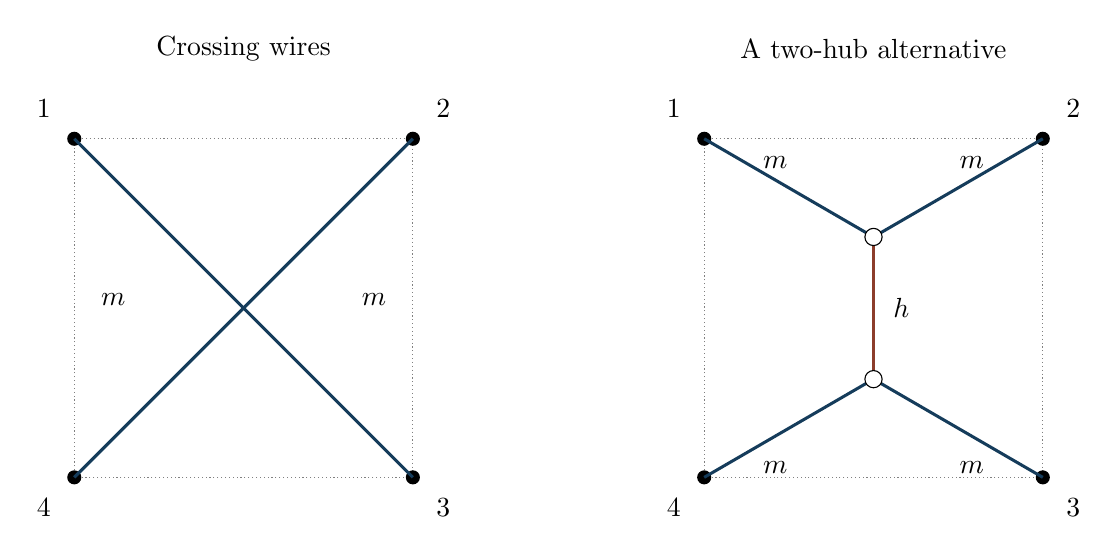
\begin{tikzpicture}[x=2.15cm,y=2.15cm,
  wire/.style={draw=wireblue,line width=1.1pt},
  terminal/.style={circle,fill=black,inner sep=1.8pt},
  hub/.style={circle,draw=black,fill=white,inner sep=2.2pt}]
  \foreach \shift in {0,8} {
    \begin{scope}[xshift=\shift cm]
      \draw[gray,densely dotted] (-1,1)--(1,1)--(1,-1)--(-1,-1)--cycle;
      \foreach \name/\x/\y in {1/-1/1,2/1/1,3/1/-1,4/-1/-1} {
        \node[terminal] at (\x,\y) {};
        \node at ({1.18*\x},{1.18*\y}) {\name};
      }
    \end{scope}
  }
  \draw[wire] (-1,1)--(1,-1);
  \draw[wire] (1,1)--(-1,-1);
  \node at (-.77,.05) {$m$};
  \node at (.77,.05) {$m$};
  \node at (0,1.53) {Crossing wires};
  \begin{scope}[xshift=8cm]
    \draw[wire] (-1,1)--(0,.42)--(1,1);
    \draw[wire] (-1,-1)--(0,-.42)--(1,-1);
    \draw[hubred,line width=1.3pt] (0,-.42)--(0,.42);
    \node[hub] at (0,.42) {};
    \node[hub] at (0,-.42) {};
    \node[right] at (.06,0) {$h$};
    \foreach \x/\y in {-.58/.86,.58/.86,-.58/-.94,.58/-.94}
      \node at (\x,\y) {$m$};
    \node at (0,1.53) {A two-hub alternative};
  \end{scope}
\end{tikzpicture}
\end{document}
